% !TEX root = frenetic_programmers_guide.tex

\chapter{NetKAT}

Software Defined Networking, or SDN, is a huge paradigm shift in the computing world.  
With traditional pre-SDN networking, you buy 
expensive, proprietary "boxes" from major vendors, plugging them in, configuring them, and hoping they 
meet your needs.  
But traditional networking suffers from these maladies:

\begin{itemize}
\item The devices are flexible only within narrow configuration parameters. 
Special requirements, like preventing certain kinds of devices from mobility, or configuring 
the spanning tree to prefer certain paths, are either impossible or expensive.
\item While the devices are powered by software, there's no good way to examine the underlying code or prove it's correct.  
\item Upgrades tend to be the forklift-variety, since mixing and matching old and new hardware is a dicey proposition
\ldots not to mention mixing hardware from different vendors.
\item Configuration is not easily automated. 
Solutions are often proprietary, require special programming languages, and are not interchangeable.
Because of this, modern data center virtualization is more difficult.
\item Adding support for new protocols is slow and expensive.
\end{itemize}

With SDN, data centers can step off the proprietary network treadmill.  
Its a shift similar to the personal computer revolution of the 1980's.
Before that, IBM and similar mainframes controlled the computer space, and required the same kinds of 
forklift upgrades networks do.
The IBM PC opened up the architecture to competitors, who could then design and 
build extensions
that made it more useful.
This created a snowball effect, with hardware extensions like the mouse and Ethernet cards opening the way 
for new software like Microsoft Windows and the Netscape browser.

SDN opens network devices in a similar manner, allowing them to be extended and manipulated in interesting,
user-defined ways.
Although the term SDN has been hijacked to mean many things, it most often refers to OpenFlow-based
devices and related software.
OpenFlow is an open protocol defined by the Open Network Foundation.

Frenetic is an OpenFlow controller, meaning it converses in the OpenFlow protocol to network switches.  
In turn, Frenetic exposes an API that can be used to write network programs easily.
It works with any network switch that understands the OpenFlow 1.0 protocol -- 
both hardware devices like the HP 2920 and software ``devices'' like Open vSwitch.  
So let's take a brief look at OpenFlow itself.

\section{Introduction to OpenFlow}

Every network device -- from the lowliest repeater, to firewalls and load balancers, all the way up to the most complex router -- has two conceptual layers:

\begin{description}
\item[The data plane] performs actions on packets.   
It manipulates headers, copies packets to outgoing (or egress) ports, or drops packets.
It consults control tables - MAC address tables, ARP caches, OSPF tables, etc. - to guide it.  
\item[The control plane] manipulates the control tables themselves.
People, in turn, may manipulate the control plane through configuration software.
Or packets may do it: specialized ones like OSPF neighbor exchange, ARP requests, or just examining plain ol'
packets themselves.
But the control plane never actually touches the packets.
\end{description}

The OpenFlow protocol makes the control plane \textit{programmable}.
Rather than relying on the entire program being \emph{inside} the box, you write a program that 
advises the control plane
running \emph{outside} the box.
It's like an advisor that makes arbitrarily complex control table manipulations.  
The programmable piece runs on any standard computer, and is collectively called the \textit{controller}.  

The controller can be written in any language and run on any computer \ldots the only requirement 
is it must speak the
OpenFlow protocol to the device.  
You can think of these two pieces working in a tandem through an OpenFlow conversation:

\begin{description}
\item[Switch:] I just got a packet, but I don't know what to do with it.
It came in port 3 from Ethernet mac address 10:23:10:59:12:fb and it's going to mac address 5c:fb:12:59:10:23.
\item[Controller:] OK.    
I'll memorize that the 10:23:10:59:12:fb address is on port 3.
But I don't know which port has a device with address 5c:fb:12:59:10:23.
So just send it out all ports on the switch except port 3.  
\item[Switch:] OK. \ldots Ooops, here's another packet I don't know what to do with.  
It came in port 5 from Ethernet mac address 5c:fb:12:59:10:23 and it's going to mac address 10:23:10:59:12:fb.
\item[Controller:]  Oh yeah.  
That looks like a reply.  
I'll memorize that the 5c:fb:12:59:10:23 address is on port 5.
Meanwhile, I know the destination is on port 3.  
Install a rule so all packets going to that mac address go out port 3, then forward this packet out port 3 as well.  
\item[Switch:] OK!
\item[Controller:] How many packets have went out port 3, by the way?
\item[Switch:] 82,120.
\item[Switch:] (To itself) I just saw a packet destined for Ethernet mac address 10:23:10:59:12:fb:5c, but I have a rule for dealing with it.  I'm gonna send it out port 3.  
\end{description}

OpenFlow boils down control plane functionality to a common core set of actions.
A list of rules and actions that can be handled in the device itself are kept in a \textit{flow table}.
Any complex decisions that can't be handled independently by the control plane may be offloaded to the controller.  
In a well-designed Software Defined Network, the controller gets involved only when necessary.
After all, the conversation between the device and the controller takes time, and anything that can 
eliminate this conversation makes the packets go faster.
So in the example above, a rule for any packets going to 10:23:10:59:12:fb:5c to be output on port 5 keeps all the processing on the switch, and out of the controller.  
That makes it really fast.  

So, central to the OpenFlow model is the \textit{flow table}.  
Flow tables have \textit{entries}, sometimes called \textit{flow rules}, that are consulted for making decisions.
A sample flow table might look like this:

\bigskip
\begin{tabularx}{6in}{|l|l|c|}
\hline\hline
Match & Actions & Priority
\\ \hline
dl\_src = 10:23:10:59:12:fb:5c, & OFPAT\_OUTPUT(9) & 100
\\
dl\_type = 0x806 & &  
\\ \hline
nw\_src = 128.56.0.0/16, & OFPAT\_SET\_DL\_DST(5c:fb:12:59:10:23), & 90 
\\
dl\_type = 0x800 & OFPAT\_OUTPUT(1) &
\\ \hline
Wildcard & OFPAT\_OUTPUT(Controller) & 1
\\ \hline\hline
\end{tabularx}

\bigskip

The main components of a flow entry are:

\begin{description}
\item[Matches] specifies patterns of packet header and metadata values.
OpenFlow 1.0 defines 12 different fields to match: some popular ones are the Input Port, 
the Ethernet Destination mac address, and the TCP destination port.
The match values can either be exact (like 10:23:10:59:12:fb:5c above) or wild carded (like 128.56.0.0/16 for a
particular Ip subnet).
\item[Actions] tell what to do if the match occurs,  
for example: send a packet out a port, or update packet header information, 
or send a packet to the controller. 
\item[Priorities] define the order that matches are consulted.  
When more than one entry matches a particular packet, the entry with the highest priority wins.
\end{description}

In our example above, the controller installed a flow entry matching Ethernet Destination 10:23:10:59:12:fb:5c, 
and an instruction applying the action "Output it through Port 3".

Suppose you wanted to write your own controller from scratch.  
You could do that just by talking the OpenFlow protocol.
Let's say you wrote this program in Node.js and placed it on the server "controller.example.com", 
listening on TCP port 6633.
Then you'd just point your OpenFlow network device at controller.example.com:6633.
Your program could install flow table entries into the network device over the OpenFlow protocol.

Hmmm.
Sounds pretty easy, but \ldots

\section{OpenFlow is Difficult}

From a programmer's perspective, a table looks awfully primitive.  
Tables are easy for switch hardware to interpret, and the faster they can interpret and carry 
out rules, the faster the packets travel.  
It's like machine language, where the CPU interprets simple instructions very quickly, and even in parallel.

Programming OpenFlow tables directly, you begin to find out the subtle missing details:

\begin{itemize}
\item You can only match packets with $=$.   There's no $\neq$.
\item There is an implicit AND in all match rows and an implicit OR between all rules.  You cannot 
arbitrarily place AND's and OR's in match rules.
\item You cannot matcha field against a set of values.  You have to write one rule per value.  
\end{itemize}

Because tables often have thousands of rules, they are difficult to construct and debug.  
In the programming world, \emph{modularization} aids both of these problems since smaller units of code
are easier to understand.  

OpenFlow tables have no inherent grouping mechanism, but we could simply modularize them by 
constructing small tables that do target packet processing.  Smoosh them together
into one big OpenFlow table when we're done, right?  

But as the paper \citet{frenetic} points out in section IIA, even simple modules can be difficult
to \emph{compose}.   Suppose your SDN switch needed to do two things: repeat all traffic, but drop all
HTTP packets coming from port 2 (a makeshift firewall).  The repeater table might look something like this:

\bigskip
\bigskip
\bigskip
\bigskip
\bigskip
\bigskip
\bigskip


\begin{figure}[h]
\centering
\begin{tabularx}{3.3in}{|l|l|c|}
\hline\hline
Match & Actions & Priority
\\ \hline
in\_port=1 & OFPAT\_OUTPUT(2) & 200
\\ \hline
in\_port=2 & OFPAT\_OUTPUT(1) & 100
\\ \hline\hline
\end{tabularx}
\end{figure}

\bigskip

And the firewall table might look like this:

\bigskip

\begin{figure}[h]
\centering
\begin{tabularx}{2.85in}{|l|l|c|}
\hline\hline
Match & Actions & Priority
\\ \hline
in\_port = 2, & None & 100
\\
tp\_src\_port = 80, &  & 
\\
dl\_type = 0x800, & &
\\
nw\_proto = 0x1 & &
\\ \hline\hline
\end{tabularx}
\end{figure}

If we simply smooshed the two tables together, the firewall rule would never fire because the first rule in 
the repeater table overshadows it.  In this case, reordering the priorities might work, but it's impossible to 
do this correctly without a spec to guide it.  

Finally, it's difficult to reason about OpenFlow tables.
While it's true that the set of possible packets is a finite set, it's still a large set.  One could loop
over all header values (200 bits worth in an OpenFlow 1.0 structured packet) 
and give the corresponding actions.  But it's tough to actually enumerate all these cases.

Frenetic obeys mathematically-defined rules about packets, and its algorithms are provably correct, which 
you can see in the paper \citet{DBLP:journals/corr/SmolkaEFG15} 
And as outlined in \citet{Foster:2015:CDP:2775051.2677011}, you can prove properties like loop-freeness and
connectivity about NetKAT programs.  

\section{Predicates}

No matter what controller you use, underneath it all, you still have OpenFlow tables.
So how does the Frenetic controller improve things? 

Other SDN controllers like OpenDaylight, RYU, and Beacon force you to manipulate 
OpenFlow tables directly.  
Frenetic works at a higher abstraction level.  
Instead of writing programs that directly call OpenFlow primitives, you write programs in 
the NetKAT language.

Frenetic's main job is to compile NetKAT predicates and policies into OpenFlow flow tables.  
It directly communicates with the switch hardware (southbound) and to your application (northbound).
Applications talk to Frenetic with standard HTTP, REST, and JSON.
The JSON-based NetKAT dialect is available to anyone, and any programming language that can talk HTTP and 
JSON can talk to Frenetic.
In this manual, we use the Python bindings for NetKAT because they're easy to use and extend, and they
come bundled with Frenetic.  
This saves you from dealing with the esoterica of HTTP communication and JSON formatting.  

So let's look at NetKAT predicates first.  
A \textit{predicate} is a clause used to match packets.
The base language is pretty straightforward:

\bigskip
\begin{tabularx}{\linewidth}{|c|X|}
\hline\hline
\texttt{SwitchEq($n$)} & Matches packets that arrive on switch $n$, where $n$ is the Datapath ID of the switch.  
\\ \hline
\texttt{PortEq($n$)} & Matches packets that arrive on port $n$.  Generally ports are numbered 1-$m$, where $m$ is the
number of interfaces, but they don't need to be consecutive.  
\\ \hline
\texttt{EthSrcEq($mac$)} & Matches packets whose Ethernet Mac source address is $mac$, which is a string in the standard form $nn:nn:nn:nn:nn:nn$ where the $n$'s are lowercase hexadecimal digits.
\\ \hline
\texttt{EthDstEq($mac$)} & Matches packets whose Ethernet Mac destination address is $mac$.
\\ \hline
\texttt{VlanEq($vlan$)} & Matches packets whose VLAN is $vlan$, and integer from 1-4096.  Packets without a VLAN are never matched by this predicate.
\\ \hline
\texttt{VlanPcpEq($p$)} & Matches packets whose VLAN Priority Code Point is $p$.  Packets without a VLAN are never matched by this predicate.
\\ \hline
\texttt{EthTypeEq($t$)} & Matches packets whose Ethernet Type is $t$, where t is a 32 bit integer.  Popular values of $t$ are 0x800 for IP and 0x806 for ARP.  
\\ \hline
\texttt{IPProtoEq($p$)} & Matches packets whose IP Protocol is $p$, a number from 0-255.  
Popular values are 1 for ICMP, 6 for TCP and 17 for UDP.  
This match only makes sense when EthTypeEq(0x800, 0x806) (IP or ARP). 
\\ \hline
\texttt{IPSrcEq($addr$, $mask$)} & Matches packets whose IP source address is $addr$.  
If $mask$ is provided, a number from 1-32, this matches all hosts on a network whose first $mask$ bits match the host.
If it's omitted, the entire address is matched -- i.e. only one IP host.  
This match only makes sense when EthTypeEq(0x800, 0x806) (IP or ARP). 
\\ \hline
\texttt{IPDstEq($addr$, $mask$)} & Matches packets whose IP destination address is $addr$.  
Follows same rules as IpSrcEq.
\\ \hline
\texttt{TCPSrcPortEq($p$)} & Matches packets whose TCP source port is $p$, an integer from 0-65535.
\\ \hline
\texttt{TCPDstPortEq($p$)} & Matches packets whose TCP destination port is $p$, an integer from 0-65535.
Popular values are 80 for HTTP, 22 for SSH, and 443 for SSL.  
\\ \hline\hline
\end{tabularx}

\bigskip
If you're familiar with OpenFlow, this list should look familiar to you -- it's the same list of fields you can 
use in an OpenFlow flow table.
One special case is SwitchEq, matching a switch id, which we'll talk about in a second.  

Unlike OpenFlow matches, NetKAT predicates can contain a list of values.  There is an explicit OR between 
the values, so only one value needs to match.  The following are equivalent predicates (the \netkat{|} means
OR, as we'll see shortly):

\begin{minted}{python}
PortEq(1) | PortEq(2) | PortEq(3)
PortEq(1, 2, 3)
PortEq( [1,2,3] )
\end{minted}

You can use boolean operators to combine predicates into bigger ones:

\bigskip
\begin{tabularx}{\linewidth}{|c|X|}
\hline\hline
\texttt{$p1$ \& $p2$} & Matches packets that satisfy $p1$ AND $p2$
\\ \hline  
\texttt{And([$p1$, $p2$, \ldots, $pn$])} & 
Matches packets that satisfy all the predicates: $p1$ \& $p2$ \& \ldots \& $pn$
\\ \hline  
\texttt{$p1$ $\vert$ $p2$} & Matches packets that satisfy $p1$ OR $p2$
\\ \hline  
\texttt{Or([$p1$, $p2$, \ldots, $pn$])} & 
Matches packets that satisfy one of the predicates: $p1$ $\vert$ $p2$ $\vert$ \ldots $\vert$ $pn$
\\ \hline  
\texttt{\textasciitilde $p1$} & Matches packets that DO NOT satisfy $p1$
\\ \hline  
\texttt{Not($p1$)} & Synonym for \texttt{\textasciitilde $p1$}
\\ \hline\hline
\end{tabularx}

\bigskip

The precedence is the same as for most Boolean operators in normal programming languages: 
\netkat{Not}, then \netkat{And}, then \netkat{Or}.  

As a shortcut, each of the field-matching predicates \netkat{FieldEq} has an analagous \netkat{FieldNotEq}
predicate which matches all values \emph{except} the given ones.  

So here are some examples in Python code:

\begin{minted}{python}
import frenetic
from frenetic.syntax import *

# Note this program doesn't actually do anything

# Match packets from a particular mac address
src_match = EthSrc("10:23:10:59:12:fb:5c")

# Match packets from a particular port that are either IP or ARP packets
port_ip_arp_match = PortEq(9) & EthType(0x800, 0x806)

# Matches packets from a particular port on switches 2 or 3 only
port_switch_match = PortEq(8) & SwitchEq(2, 3)

# Matches packets from all ports except 2 or 3
non_router_match = PortNotEq(2, 3)

# Matches broadcast packets or packets from a particular port 
# or packets with a particular Vlan
all_criteria = [ EthSrc("ff:ff:ff:ff:ff:ff"), PortEq(1), VlanEq(2345) ] 
brd_or_port_match = Or( all_criteria ) 

\end{minted}

Note that you can assign predicates to Python variables.  They are never actually matched against packets
in Python, however \ldots they are always interpreted on the switch itself as part of a rule.

One predicate requires some explanation: \netkat{SwitchEq}.  
An OpenFlow flow table belongs to one and only one switch, but a NetKAT program belongs to every
switch connected to that controller.  
So a predicate tagged with \netkat{SwitchEq} will limit a particular match to a particular switch.
Any predicates that don't have a \netkat{SwitchEq} predicate will apply to \textit{all} switches in the network.

Finally, there are a few special predicates:

\bigskip
\begin{tabularx}{\linewidth}{|c|X|}
\hline\hline
\texttt{true} & Matches all packets
\\ \hline  
\texttt{Id()} & Matches all packets
\\ \hline  
\texttt{false} & Matches no packets
\\ \hline  
\texttt{Drop()} & Matches no packets
\\ \hline\hline
\end{tabularx}
\bigskip

Why would you need these?  
They're useful for "catch all" rules that appear last in a list.
A good example is our repeater, where we had an id rule that matched all packets and
forwarded them to the controller.

\section{Policies}

NetKAT predicates are powerless by themselves.  
To make them work, you need to use them in NetKAT \textit{policies}.
A policy is like a command, and policies are compiled down to OpenFlow actions, 
and are used in table rules or the \python{packet_out} command.  
But just as NetKAT predicates are more powerful than OpenFlow matches, NetKAT policies are more
powerful than OpenFlow action lists.

\bigskip
\begin{tabularx}{\linewidth}{|c|X|}
\hline\hline
\texttt{Filter($p$)} & Select packets that match NetKAT predicate p, and quietly forget the rest  
\\ \hline
\texttt{id} & Lets all packets through.  Equivalent to \texttt{Filter(True))}  
\\ \hline
\texttt{drop} & Drops all packets.  Equivalent to \texttt{Filter(False))}  
\\ \hline
\texttt{SetPort($n$)} & Set the output port for the packet to port $n$.    
\\ \hline
\texttt{SendToController($tag$)} & Send packet to controller with tag $tag$    
\\ \hline
\texttt{SetEthSrc($mac$)} & Set Ethernet Mac source address to $mac$
\\ \hline
\texttt{SetEthDst($mac$)} & Set Ethernet Mac destination address to $mac$.
\\ \hline
\texttt{SetVlan($vlan$)} & Set packet VLAN to $vlan$.  Note this is not a Vlan push - it overwrites whatever 
Vlan is in the packet (if there is one).  
\\ \hline
\texttt{SetVlanPcp($p$)} & Set VLAN Priority Code Point to $p$.
\\ \hline
\texttt{SetEthType($t$)} & Set Ethernet Type to $t$, where t is a 32 bit integer.
\\ \hline
\texttt{SetIPProto($p$)} & Set IP Protocol to $p$.    
\\ \hline
\texttt{SetIPSrc($addr$)} & Set IP source address to $addr$.  Note there is no mask here, as in the equivalent predicate.  
\\ \hline
\texttt{SetIPDst($addr$)} & Set IP destination address to $addr$.  
\\ \hline
\texttt{SetTCPSrcPort($p$)} & Sets TCP source port to $p$.
\\ \hline
\texttt{SetTCPDstPort($p$)} & Sets TCP destination port to $p$.  
\\ \hline\hline
\end{tabularx}
\bigskip

Note that \texttt{Set} policies mirror each Eq predicate, so for example the predicate \texttt{VlanEq($vlan$)} has a matching
\texttt{SetVlan($vlan$)}.
The exception is \texttt{Switch}.  
You can't just set the Switch to some ID -- that would be analogous to teleporting a packet from one 
switch to another!
To send a packet to a different switch, you also use \texttt{Send}, but you are restricted to switches that are directly
connected to the current switch, and you must know out which port to send it.
We'll cover strategies for dealing with this in Chapter \ref{spanning_tree}.
 
And just as you can combine predicates with Boolean operators, you can combine policies with NetKAT 
policy operators:

\bigskip
\begin{tabularx}{\linewidth}{|c|X|}
\hline\hline
\texttt{$pol1$ | $pol2$} & Copy the packet and apply both $pol1$ and $pol2$ to it.   
This is called \textit{parallel composition}.
\\ \hline  
\texttt{Union([$pol1$, $pol2$, \ldots $poln$])} & 
Copy the packet $n$ times and apply policy $pol[i]$ to copy $i$.
Equivalent to \texttt{$pol1$ | $pol2$ | $poln$}
\\ \hline  
\texttt{$pol1$ >> $pol2$} & Apply the policy $pol1$ to the packet, then apply $pol2$ to it
This is called \textit{sequential composition}.
\\ \hline  
\texttt{Seq([$pol1$, $pol2$, \ldots $poln$])} & 
Apply each of the policies $pol1$, $pol2$, \ldots, $poln$ to the packet, in order 
Equivalent to \texttt{$pol1$ >> $pol2$ >> \ldots $poln$}
\\ \hline  
\texttt{IfThenElse($pred$, $pol1$, $pol2$)} & If packet matches predicate $pred$, then apply policy $pol1$, or else
apply $pol2$.  
Either $pol1$ or $pol2$ is applied, but never both.
\\ \hline\hline
\end{tabularx}

\bigskip

The \texttt{>>} should look familiar to C++ programmers. 
Like in C++, the \texttt{>>} operator changes a piece of data, then forwards it to the next step in the chain, one
after the other.
It's especially helpful in I/O, where you build a string from pieces, then send it to the output device (file or screen) as the
last step.

The $\vert$ symbol is somewhat like the equivalent in UNIX shell programming: the components run in parallel.
However, unlike $\vert$, in NetKAT you are actually running separate copies of each policy without any connections
between them.
In other words, you don't send packets from the output of one into the input of another.
(Note that $\vert$ is also the OR symbol in NetKAT predicates, but NetKAT distinguishes between the two in
its parser.)

The difference between sequential and parallel composition is subtle, and we'll talk about it more in
Section \ref{section:combining}

\section{Commands and Hooks}

Just like NetKAT predicates, NetKAT policies don't do anything by themselves.
We need to install policies as switch rules or use them in \netkat{pkt_out} operations.  

And so we come to the last level of a net app: commands and hooks.
Commands are instructions from the net app to the switches (via Frenetic).  
OpenFlow calls these \emph{controller-to-switch messages}.  
Hooks are instructions from the switches to the net app (again, via Frenetic), and OpenFlow
calls these \emph{switch-to-controller messages.}

The commands are:

\bigskip
\begin{tabularx}{\linewidth}{|c|X|}
\hline\hline
\texttt{pkt\_out($sw$, $payload$,} & Send a packet out switch with DPID $sw$.  We'll describe 
\\
\texttt{$plist$, $inport$)} & this in detail below.
\\ \hline  
\texttt{update($policy$)} & 
Update all switches with the given NetKAT policy.
This is the equivalent of setting the OpenFlow flow tables of all switches in one shot.  
\\ \hline  
\texttt{port\_stats($sw$, $port$)} & Get statistics for a particular switch and port. 
\\ \hline  
\texttt{query($label$)} & Get user-defined statistics associated with a particular label. 
We'll cover this in Chapter \ref{chapter:statistics}.
\\ \hline  
\texttt{current\_switches()} & Gets a list of DPID's of all current, operating switches, and the operating
ports for each.  
This is most useful in the \texttt{connected()} hook.  
\\ \hline  
\texttt{config($compiler\_options$)} & Set Frenetic compiler options.  
This is an instruction to Frenetic, not the switch. 
\\ \hline\hline
\end{tabularx}

\bigskip
You call commands through Python method calls, e.g. \texttt{self.update($policy$)}.  
The hooks are:

\bigskip
\begin{tabularx}{\linewidth}{|c|X|}
\hline\hline
\texttt{connected()} & Called when Frenetic has finished startup and some (perhaps not all) 
switches have connected to it. 
\\ \hline
\texttt{packet\_in($sw$, $port$, $payload$)} & 
Called when 
a packet has arrived on switch $sw$, port $port$ and a matching policy had a \texttt{SendToController} action
 This is described in detail below.
\\ \hline  
\texttt{switch\_up($sw$)} & Called when a switch has been initialized and is ready for commands.  
Some switches send this message periodically to verify the controller is operational and reachable.
\\ \hline  
\texttt{switch\_down($sw$)} & Called when a switch has been powered-down gracefully.
\\ \hline  
\texttt{port\_up($sw$, $port$)} & Called when a port has been activated.
\\ \hline  
\texttt{port\_down($sw$, $port$)} & Called when a port has been de-activated - most of the time, that means the link
status is down, the network cord has been unplugged, the host connected to that port has been powered-off,
or the port has been reconfigured.
\\ \hline\hline
\end{tabularx}

\bigskip
Your net app may be interested in one or more of these hooks.
To add code for a hook, you write a \emph{handler} which implements the hook's signature.
Following Python conventions, it must be named exactly the same as the hook.
However, you don't need to provide handlers for every hook.
If you don't provide one, Frenetic uses its own default handler -- in the case of \texttt{connected()}, for example, it
merely logs a message to the console.  

We'll see most of these commands and hooks used in the next few chapters.  
But since \texttt{pkt\_out()} and \texttt{packet\_in()} are the most
crucial for net apps, we'll describe them first here.

\subsection{The packet\_in Hook}
\label{introduction:packet_in}

\texttt{packet\_in()} is used to inspect network packets.  
Note that \emph{not all packets} coming in through all switches 
arrive here -- indeed, if they did, your controller would be
horribly slow (as our Repeater example is, but we'll see how to improve it in a bit.)
A packet will be sent to the controller when it matches a rule with a \netkat{SendToController} policy.  

Once at the controller, Frenetic will deliver the packet to \texttt{packet\_in()}. 
The default handler will simply log a message and drop the packet, but of course that's not very interesting.
The handler \python{packet_in} is called with three parameters:

\bigskip
\begin{tabularx}{6in}{|c|X|}
\hline\hline
\texttt{sw} & The DPID of the switch where the packet arrived.
\\ \hline
\texttt{port} & The port number of the port where the packet arrived.
\\ \hline
\texttt{payload} & The raw packet data.
\\ \hline\hline
\end{tabularx}

\bigskip
There are two formats for the packet data: \emph{buffered} or \emph{unbuffered}.
Most switches will only send unbuffered data, meaning the entire network packet - header and data - will be 
transferred to the controller.
We'll talk about buffering in Section \ref{intro:buffering}.

If you don't need to examine any packet data, you can simply drop $packet$, or pass it directly to \texttt{pkt\_out},
as we did in our Repeater app:

\begin{minted}{python}
...
class RepeaterApp(frenetic.App):

...
    def packet_in(self, dpid, port_id, payload):
        out_port = 2 if port_id = 1 else 1
        self.pkt_out(dpid, payload, [ Output(Physical(out_port_id)) ] )

...
\end{minted}

Here, we merely send the payload out unchanged.  
If it came in as buffered data, it will be sent out as buffered data.
If it came in unbuffered, it will be sent out unbuffered.  
Pretty simple.

If you need to examine the payload, you'll need some assistance.
The payload is the raw network packet data, not parsed or translated at all.
So for the Ethernet Source address, for example, you'd need to examine bytes 14 through 19 
(byte ordering starts at 0).  
Working at this low-level is exceedingly error prone, so Frenetic leverages the RYU Packet library.
RYU is an open source project spearheaded by NTT (Nippon Telephone and Telegraph) and its Python packet
parsing library is very solid and complete.

Frenetic provides a simple API on top of RYU Packet.

\begin{minted}{python}
# You must import the proper protocol from the RYU packet library to use it
from ryu.lib.packet import ethernet, arp
...
    def packet_in(self, dpid, port_id, payload):
        ethernet_packet = self.packet(payload, 'ethernet')
        src_mac = ethernet_packet.src
        if ethernet_packet.ethertype = 0x806:
          arp_packet = self.packet(payload, 'arp')
          src_ip = arp_packet.src_ip

...
\end{minted}

\python{p = self.packet(payload, protocol)} turns the raw 
\python{payload} into a parsed packet of type \python{protocol}.  
From there, the fields of \python{p} are the parsed values of that protocol.  
You can think of \python{p} as a view into \python{payload} with the 
\python{protocol} lens attached.  
In the example above, for example, \python{payload} is both an Ethernet packet and an ARP packet, and the 
variables \python{ethernet_packet} and \python{arp_packet} provide respective views into it.   
If \python{payload} is not parseable into that protocol, \texttt{None} is returned.  

http://ryu-zhdoc.readthedocs.org/en/latest/library\_packet\_ref.html 
contains a complete reference for RYU packets. 
Here are the most popular protocols and fields:

\subsubsection{ethernet}

\bigskip
\begin{tabularx}{\linewidth}{|c|X|}
\hline\hline
\texttt{dst} & Destination mac address string, formatted as "08:60:6e:7f:74:e7" 
\\ \hline
\texttt{src} & Source mac address string 
\\ \hline
\texttt{ethertype} & Ethernet frame type.  
Popular values are 0x800 for IP version 4, or 0x806 for ARP.  
\\ \hline\hline
\end{tabularx}

\bigskip
Constructor: \texttt{ethernet.ethernet(dst, src, ethertype)}

\subsubsection{vlan}

\bigskip
\begin{tabularx}{\linewidth}{|c|X|}
\hline\hline
\texttt{vid} & VLAN id 
\\ \hline
\texttt{pcp} & Priority Code Point 
\\ \hline
\texttt{ethertype} & Ethernet frame type.  
The outer Ethernet packet has ethertype 0x8100, so this is the ethertype of the packet's data.
\\ \hline\hline
\end{tabularx}

\bigskip
Constructor: \texttt{ethernet.vlan(pcp, vid, ethertype)}

\subsubsection{ipv4}

\bigskip
\begin{tabularx}{\linewidth}{|c|X|}
\hline\hline
\texttt{proto} & The IP version 4 protocol.  
Popular values are  6 for TCP and 17 for UDP.
\\ \hline
\texttt{src} & Source address, a 32 bit integer 
\\ \hline
\texttt{dst} & Destination address, a 32 bit integer
\\ \hline\hline
\end{tabularx}

\bigskip
Constructor: \texttt{ipv4.ipv4(proto, src, dst)}

\subsubsection{arp}

\bigskip
\begin{tabularx}{\linewidth}{|c|X|}
\hline\hline
\texttt{opcode} & Popular values are \texttt{arp.ARP\_REQUEST} and \texttt{arp.ARP\_REPLY}.  
\\ \hline
\texttt{src\_mac} & Source mac address string, formatted as "08:60:6e:7f:74:e7"  
\\ \hline
\texttt{src\_ip} & Source IP address, a 32 bit integer  
\\ \hline
\texttt{dst\_mac} & Destination mac address string  
\\ \hline
\texttt{dst\_ip} & Destination IP address  
\\ \hline\hline
\end{tabularx}

\bigskip
Constructor: \texttt{arp.arp\_ip(opcode, src\_mac, src\_ip, dst\_mac, dst\_ip)}

\subsection{The pkt\_out Command}

\texttt{pkt\_out} is used to send out packets.  
Most of the time, the packets you send are packets you received through \texttt{packet\_in}.
But there's nothing stopping from you sending arbitrarily-constructed packets from here as well.  

The command takes the following parameters:

\bigskip
\begin{tabularx}{\linewidth}{|c|X|}
\hline\hline
\texttt{sw} & The DPID of the switch from where the packet should be sent.
\\ \hline
\texttt{payload} & The raw packet data, wrapped in a 
Buffered or Unbuffered object type.
\\ \hline
\texttt{policy\_list} & Python list of NetKAT policies (actions) to apply to the packet data.
\\ \hline
\texttt{in\_port} & Port ID from which to send it.
This parameter is optional, and only applies to buffered packets presumably sitting at a particular port on
the switch waiting to be released.
\\ \hline\hline
\end{tabularx}

\bigskip

The \python{policy_list} effectively tells the switch how to act on the packet.  
Most NetKAT policies are usable here including \texttt{SetIPSrc} and \texttt{SendToController}.  The
exceptions are:

\begin{itemize}
  \item \texttt{Filter} is not usable.  To optionally send or not send packets, use the packet parsing library
  from RYU to examine the packet and make decisions.  
  \item \texttt{SetPort} is not available, but \texttt{Output(Physical($p$))} can be substituted.  The 
  difference is subtle.  \texttt{SetPort} can be used anywhere in a policy sequence, and can be followed
  by more packet modifications.  \texttt{Output} sends the packet out immediately, and according to OpenFlow
  it is always the last action executed if present.   
  \item Only simple policies are doable, so you can't use policy operators like \texttt{Union}, \texttt{Seq} 
  and \texttt{IfThenElse}.  Instead, you can send multiple policies in a list, where there's an implied \texttt{Seq} 
  operator between them.
\end{itemize}

What if you want to modify a packet before sending it out?  
There are actually two ways to do it, each appropriate for a particular use case:

\begin{description}
  \item[Direct Modification] where you set particular data in the packet itself, reserialize it through RYU's packet
  library API, and send it in \python{payload}.  
  This is the only way to modify data that's not accessible to a NetKAT policy - e.g. the IPv4 source address is
  settable by NetKAT policy \texttt{SetIPv4}, but there's no equivalent policy for the ARP opcode.  
  Direct modification is only available for unbuffered packets.
  \item[Policy Modification] is achieved through the Policy list, and is limited to modification through NetKAT
  policies.
  It can be done on buffered or unbuffered packets.
\end{description}

In general, Policy Modification is preferable since it works on all packets, and saves you the costly step of parsing and 
reserializing the packet in the controller.
For example, a common routing function is to change the destination MAC address for a next hop router.
Here's an example of doing this with Policy Modification:

\begin{minted}{python}

    def packet_in(self, dpid, port_id, payload):
        (next_hop_mac, next_port) = calculate_next_hop(payload)
        self.pkt_out(dpid, new_payload, 
          [ SetEthDst(next_hop_mac), Output(Physical(next_port)) ]
        )	

\end{minted}

For those times when you need Direct Modification, here's an example of how to do it:

\begin{minted}{python}
from ryu.lib.packet import ethernet, arp
...

    def payload(self, e, pkt):
        p = packet.Packet()
        p.add_protocol(e)
        p.add_protocol(pkt)
        p.serialize()
        return NotBuffered(binascii.a2b_base64(binascii.b2a_base64(p.data)))

    def packet_in(self, dpid, port_id, payload):
        ethernet_packet = self.packet(payload, 'ethernet') 
        arp_packet = self.packet(payload, 'arp')
        # Flip a request into a reply and vice versa
        arp_packet.opcode =  \ 
          arp.ARP_REPLY if arp_packet.opcode == arp.ARP_REQUEST \
          else arp.ARP_REPLY
	    # Reserialize it back into a raw packet
        new_payload = self.payload(ethernet_packet, arp_packet)
        self.pkt_out(dpid, new_payload, [ Output(Physical(1)) ])	
...
\end{minted}

You can also create packets from scratch with a variation of Direct Modification.  
First create the packet views with standard RYU Packet library constructors.
Then just call \texttt{self.payload()} on them to create the raw packet and send it.  

\begin{minted}{python}
from ryu.lib.packet import ethernet, arp
...
    def send_arp_reply(port, src_mac, dst_mac, src_ip, dst_ip):
        # Immediately send an ARP reply when a port comes up.
        e = ethernet.ethernet(dst=dst_mac, src=src_mac, ethertype=0x806)
        a = arp.arp_ip(arp.ARP_REPLY, src_mac, src_ip, dst_mac, dst_ip)
	    # Serialize it into a raw packet
        new_payload = self.payload(ethernet_packet, arp_packet)
        self.pkt_out(dpid, new_payload, [ Output(Physical(port)) ])	
...
\end{minted}

\subsection{Buffering}
\label{intro:buffering}

Packet buffering is often a settable option in a switch's OpenFlow configuration.  It's 
especially useful when packets are large, as in Jumbo Frames.  Most switching decisions made in 
the controller look only at the packet headers, not the data, so why should you have to send it?  By buffering the
entire packet, the switch only sends the headers to the controller.  

A buffered Packet Out \emph{must always} be preceded by a buffered Packet In.  That's because you need 
to send back two things:
the incoming port id, and the buffer id.  The switch actually has separate buffer lists 
for every port on the switch, and 
sending it back with the proper port helps it match it to the correct buffer.   
This sequence diagram shows how it commonly works:

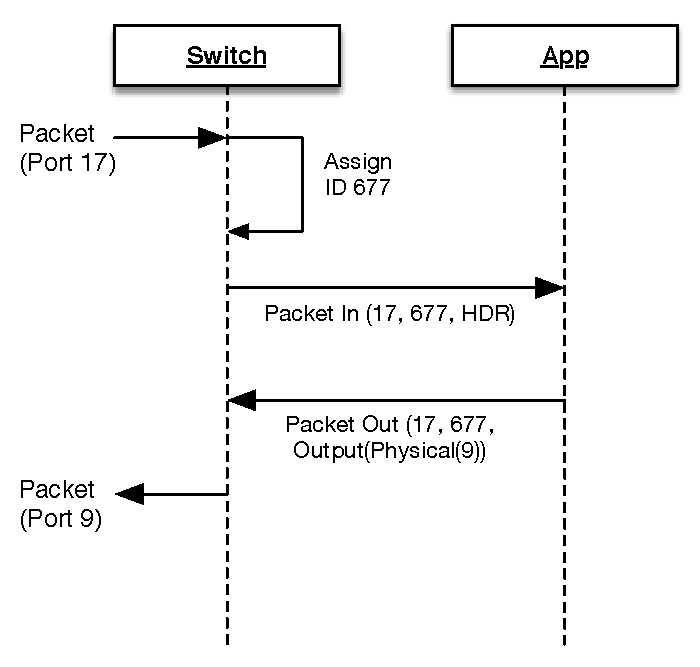
\includegraphics{buffered_pkt_happy_path}

Here, the HDR is the first 128 bytes of the packet, enough to hold the Ethernet and IP header information,
typically.  The app doesn't send any of this header information back to the switch - just the instruction
\texttt{Output(Physical(9))} to direct the switch's data plane.

What if we \emph{never} send back the Packet Out?  Buffer contents are not held indefinitely -- they timeout after a 
certain period.  At that point, the buffered packet will drop out.
If we send a Packet Out for that buffer after the timeout period, the Packet Out will generate an error (which
Frenetic ignores).    A similar fate awaits Packet Outs that fabricate a random buffer id, or send it to the
wrong port.  

So where is the buffer id in the \texttt{PacketOut} call?  It's embedded in the \texttt{payload} object.
When a \texttt{PacketIn} delivers a buffered payload, you can simply it send it back out the \texttt{PacketOut}
call, which sends the buffer id along with it.  

\section{OpenFlow Constructs Not Supported by NetKAT}

NetKAT supports the most popular features of OpenFlow 1.0.  But there a few things it doesn't do:

\begin{itemize}
\item It can't output to special pseudo-ports NORMAL, FLOOD, etc.  The semantics of sending to these ports
depends on the spanning tree, VLAN's, and other settings that NetKAT is not aware of, so it cannot reason
about them. 
\item It can't set the size for buffered packet data in \texttt{SendToController}.  All buffered packets
get sent with the default 128 bytes, usually enough to encapsulate the header information.
\item It can't retrieve flow table counters.  Since one NetKAT policy may expand to many OpenFlow rules, or even 
be optimized to OpenFlow Rules, there is no good way to map and retrieve this data.
\item Frenetic must talk to switches through an unsecured channel.  TLS is not supported.
\item Most controller-to-switch messages like Features, Configuration or Barrier are not supported.
\item Some switch-to-controller messages like Error, Flow Removed and Vendor are ignored by Frenetic. 
\item Some OpenFlow actions are not supported, like Enqueue.   
\end{itemize}

We haven't discussed some implemented features like Statistics yet, but those will be described in chapter \ref{chapter:statistics}.